\chapter{Обзор литературы} \label{ch:ch1}
\section{Приложения квантовой информатики} \label{sec:ch1/sec1}

Квантовая информатика - область знаний, сочетающая в себе элементы теории информации и фотоники. В качестве базовой единицы в рамках квантовой информатики используются квантовые биты, или кубиты, - системы, которые могут находиться в состоянии суперпозиции и применяться для хранения, вычисления и передачи информации. Одним из перспективных направлений являются квантовый вычислитель и квантовая память - основные составляющие квантового компьютера - принципиально нового типа вычислительных устройств, работающего на фундаментальных принципах квантовой механики. Передача квантового состояния на различные расстояния, или квантовая телепортация, - другое перспективное приложение квантовой информатики. Генерация симметричной битовой последовательности квантовым методом, или квантовая рассылка ключа (КРК), сформировалось как научное направление в 80-ых годах 20-го века. Данное направление является передовым с точки зрения прикладного применения. В системах квантовой коммуникации (СКК) за счет использования квантовых состояний два и более легитимных абонентов могут осуществлять рассылку симметричных битовых последовательностей, которые в последствии могут быть использованы в качестве ключей для кодирования информации, таким образом, что любые попытки несанкционированного доступа нелегитимного пользователя в канал связи будут обнаружены по возросшему уровню ошибок.


Прикладные аспекты квантовой информатики вызывают повышенный интерес в последние годы. В качестве примера, основоположники квантовой рассылки ключа и квантовой криптографии Ч. Беннет и Ж. Брассар являлись основными фаворитами на получение Нобелевской премии 2012 года с их работами по открытию и экспериментальному подтверждению квантовой телепортации [4].  

Системы квантовой коммуникации активно разрабатываются во всём мире. Положительные результаты исследований и достижение ключевых параметров система такого класса, удовлетворяющих потребительские запросы позволили перейти со стадии экспериментальных исследований на стадию коммерческого распространения. Также наблюдается рост количества патентов на разработки и публикаций в рецензируемых журналах в данной сфере [6,7].

В настоящий момент исследования в области квантовой рассылки ключа находятся в фазе стандартизации и сертификации в соответствии с потребностями целевых структур и доработки устройств в соответствии с этими регламентами. В качестве предшествующих этапов развития технологии можно выделить: формирование основных принципов функционирования систем подобного рода, а также ряда методов генерации и обработки квантовых состояний, и разработка протоколов квантового распределения ключа. На сегодняшний день разработки ведутся с целью повышения технических параметров и характеристик СКК: увеличения скорости формирования кодирующих битовых последовательностей и повышения дистанции линии связи между абонентами, участвующими в распределении ключа, повышение пропускной способности каналов за счет технологии спектрального уплотнения, уменьшения уровня шумов и воздействия внешней среды на оптические сигналы, а также интеграция в волоконно-оптические линии связи телекоммуникационного стандарта и работоспособность в полевых, а не лабораторных условиях. Отдельным интересным направлением развития технологии является адаптация систем к условиям работы в открытом пространстве (земля-воздух, земля-космос). Прорывным стал запуск спутника с системой квантовой коммуникации на борту для осуществления процедуры КРК на межконтинентальном уровне.

%%%%%%%%%%%%%%%%%%%%%%%%%%%%%%%%%%%%%%%%%%%%%%%%%%%%%%%%%%%%%%%%%%%%%%%%%%%%%%%%%%%%%%%%%%%%%%%%%%%%%%%%%%%%%%%%%%

\section{Системы квантовой коммуникации} \label{sec:ch1/sec2}

В современных методах защиты передаваемой информации можно выделить два критических места:
\begin{enumerate}
	\item Условная устойчивость алгоритмических методов кодирования и шифрования информации. Предполагается, что для взлома современных алгоритмов шифрования, злоумышленнику потребуется значительное количество времени, так как он не обладает достаточными вычислительными ресурсами [8].
	\item Развитие квантовых вычислений и предпосылки к появлению квантового компьютера, обладающего необходимыми вычислительными ресурсами, для того чтобы раскрыть зашифрованную алгоритмическими методами информацию за короткое время [9].
\end{enumerate} 


 <<Метод одноразового блокнота>>, предложенный Ж. Вернамом [10], удовлетворяет необходимым требованиям к системам кодирования и защиты информации. В основе лежит принцип обмена между легитимными абонентами <<абсолютно стойкими ключами>> (АСК). Ключ можно назвать абсолютно стойким при выполнении ряда требований:

\begin{enumerate}
	\item Одноразовое использование;
	\item Длина кодирующей последовательности равна или превосходит длину шифруемого сообщения;
	\item Ключ абсолютно случаен;
	\item Ключ известен только легитимным абонентам.
\end{enumerate}


В связи с накладываемыми на АСК требованиями возникает проблема распределения между доверенными лицами. Одно из возможных решений основывается на фундаментальных физических принципах.


Таким образом, квантовая рассылка ключа (КРК) - область в квантовой информатике, направленная на решение проблемы распространения АСК между доверенными абонентами [12].


Уникальность КРК заключается в том, что условие доступности АСК только легитимным пользователям достигается за счет фундаментальных принципов квантовой физики [12, 13]. А именно: измерение, изменение, усиление, копирование или разделение одних параметров квантовой системы без внесения изменения в другие [14]. Благодаря количеству срабатываний, фиксирующих корреляцию состояний, определяется наличие злоумышленника в линии связи.


Принципиальная схема СКК (рис.\ref{fig:Fig_1}) включает в себя модуль получателя, именуемый Бобом (Bob), модуль отправителя, именуемый Алисой (Alice), два связывающих их тракта: квантовый канал и открытый (служебный) канал. Также обычно предполагается наличие злоумышленника Евы (Eve-eavesdropper) [12].


Принципиальная схема изображена на рис. \ref{fig:Fig_1}
 \begin{figure}[ht]
  \centering
  \includegraphics {Basic_scheme.pdf}
  \caption{Принципиальная схема системы квантовой коммуникации [12]}
  \label{fig:Fig_1}
\end{figure}


Процедура КРК осуществляется по квантовому каналу, в качестве которого чаще всего применяется волоконно-оптическая линия связи, с манипуляцией параметрами квантовых систем (одиночных фотонов). Служебный канал является открытым и доступным злоумышленнику и используется для осуществления протокола выработки ключа, выяснения легитимными пользователями изменений статистики отсчетов и коррекции ошибок в первичном (<<сыром>>) ключе, переданном по квантовому каналу связи [13].

%%%%%%%%%%%%%%%%%%%%%%%%%%%%%%%%%%%%%%%%%%%%%%%%%%%%%%%%%%%%%%%%%%%%%%%%%%%%%%%%%%%%%%%%%%%%%%%%%%%%%%%%%%%%%%%%%%

\section{Протоколы квантовой коммуникации} \label{sec:ch1/sec3}

Протоколом квантового распределения ключа называется алгоритм формирования кодирующих битовых последовательностей квантовыми методами. В результате передачи однофотонных состояний с измененным параметром от модуля отправителя к модулю получателя образуется набор скоррелированных бит. Первыми считаются протоколы BB84 и B92, разработанные пионерами КРК. В основе первого лежит применение 4 квантовых состояний, в качестве которых используются, например, поляризационные степени свободы фотонов, по два в каждом из двух базисов - вертикально-горизонтальном и диагональном [12]. Второго - кодирование в 2 состояния, ортогональных друг другу, в качестве которых традиционно используется фазовая отстройка сигналов либо относительно друг друга, либо относительно задающего оптического сигнала. Один из методов формирования кубитов -  кодирование с использованием интерферометрических схем, например Маха-Цендера, в результате чего формируется фазовая отстройка [13]. 

Формирование ключа происходит следующим образом: сначала модуль отправителя модулирует световой импульс с внесением фазового сдвига случайным образом, выбирая между двумя возможными состояниями 0 или $\pi$. Отправитель и получатель имеют предварительную договоренность, какие значения фазы будут соответствовать 0 и 1 в формируемой последовательности. Оптический импульс отправляется в квантовый канал, например ВОЛС. При поступлении на модуль получателя происходит аналогичная модуляция, однако фазовый сдвиг выбирается случайным образом независимо от отправителя. В результате второй модуляции происходит интерференция оптических импульсов. Детектор одиночных фотонов (ДОФ) регистрирует результат интерференции этих импульсов. В случае, когда результат интерференции носит конструктивный характер, то приёмный модуль верно угадал фазу (мы не учитываем влияние случайных шумовых собственных срабатываний ДОФ). Результат срабатывания фиксируется и соотносится с состоянием, которое применялось при модуляции в данный такт. Полученный бит интерпретируется как 0 или 1 в зависимости от начальной договоренности. В случае деструктивной интерференции возможны два случая: или состояние, использованное в приёмном блоке в данный такт не совпадает с состоянием, использованным отправителем, или в этот временной отсчет не было послано ни одного фотона, либо фотон не дошел до приёмного блока ввиду затуханий в линии связи. Процедура повторяется для каждого светового импульса, следующего с заданной периодичностью (тактовой частотой). По завершению процедуры модуль получателя сообщает по служебному каналу модулю отправителя, в какие промежутки времени наблюдалась конструктивная интерференция и срабатывания ДОФ, не сообщая, какую модуляцию он использовал. Такты, в которых ДОФ не зарегистрировал импульсы, отбрасываются. Алиса по открытому служебному каналу принимает информацию о промежутках времени, когда было зафиксировано совпадение и только эти биты остаются в качестве <<сырого>> ключа. Далее производится оценка величины среднего количества ошибок по битам (QBER - quantum bit error rate). Затем при помощи процедур исправления ошибок у обоих абонентов остаются идентичные последовательности. Последним этапом является процедура усиления секретности (privacy amplification), задачей которой является симметричное изменение последовательностей, чтобы уменьшить вероятность получения ключевой информации злоумышленником.


\begin{table} [htbp]
	\centering
	\caption{Пример формирования ключа по протоколу B92.}
	\label{tab:protocol}
	\begin{tabular}{| c | c | c | c | c |}
	 \hline	Алиса                              & \multicolumn{2}{|c|}{0}   & \multicolumn{2}{|c|}{1}   \\ \hline
	  Фаза Алисы					     	   & \multicolumn{2}{|c|}{0}   & \multicolumn{2}{|c|}{1}   \\ \hline
	  \makecell{Боб выбирает \\ фазу}	    	   & 0      	                   & 180    & 0 	& 180      \\ \hline
	  \makecell{Боб детектирует \\ фотон}      & ДА                        & НЕТ    & НЕТ   & ДА       \\ \hline
	  \makecell{Алиса и Боб \\ разделяют бит}  & ДА                        & НЕТ    & НЕТ   & ДА       \\ \hline
	\end{tabular}%
\end{table}


Базовая схема B92 представлена на рисунке \ref{fig:Fig_2}. Каждое плечо распределенного в пространстве интерферометра Маха-Цендера находится у одного из абонентов.
 

 \begin{figure}[ht]
  \centering
  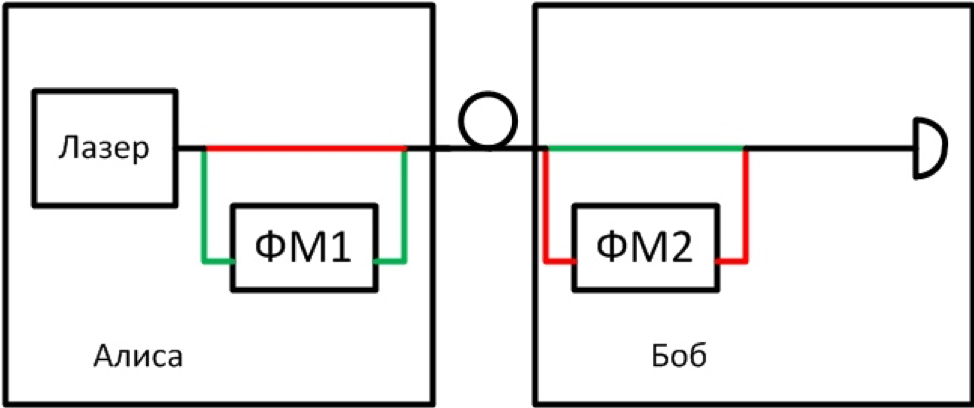
\includegraphics {Fig_2.png}
  \caption{Принципиальная схема системы квантовой коммуникации с фазовым кодированием [13]}
  \label{fig:Fig_2}
\end{figure}

Лазерный импульс в блоке отправителя делится пополам при помощи светоделителя: одна половина следует по <<короткому>> пути (красный1), а вторая половина по <<длинному>> пути (зеленый1) и проходит через первый модулятор фазы (ФМ 1). Информация кодируется внесением фазового сдвига в ФM 1. Затем импульсы распространяются по линии связи. В приёмном модуле импульсы поступают во второе плечо распределенного интерферометра, где происходит повторное разделение на две равные части и модуляция на ФМ 2. В результате чего наблюдается три вида импульсов. Первый, прошедший дважды по <<короткому>> пути (зеленый2) и последний, дважды прошедший по <<длинному>> (красный2), не несут никакой информации. Средний является результатом интерференции импульсов, прошедших пути красный1-красный2 и зеленый1-зеленый2. Для регистрации результата интерференции необходимо отделить от мощного импульса красный1-зеленый2 с помощью электро-оптического затвора ЭЗ и направить на ДОФ. Вдобавок можно использовать качестве опорного импульс красный1-зеленый2, то есть сообщать поступлении однофотонного импульса.

%%%%%%%%%%%%%%%%%%%%%%%%%%%%%%%%%%%%%%%%%%%%%%%%%%%%%%%%%%%%%%%%%%%%%%%%%%%%%%%%%%%%%%%%%%%%%%%%%%%%%%%%%%%%%%%%%

\section{Системы квантовой коммуникации на боковых частотах модулированного излучения} \label{sec:ch1/sec4}

Системы квантовой коммуникации с вынесением квантового канала на боковые частоты в результате фазовой модуляции оптической несущей частоты был предложен в [?]. Метод развивался несколькими группами в различных практически значимых направлениях. Исследовалось увеличение спектральной эффективности за счет формирования нескольких боковых частот одновременно [?]. Разрабатывались методы, решения и подходы с целью увеличения тактико-технических характеристик СКК [?]. Устройство и оптическая схема модифицировались для интегрирования в стандартное телекоммуникационное одномодовое волокно повсеместно используемое для широкополосного доступа в сеть Интернет. Преимуществом квантовой коммуникации на боковых частотах (ККБЧ) является отказ от использования традиционного интерферометра на основе Маха-Цендера, требовательного к сложной юстировке, за счет формирования интерферометра в спектре сигнала, где радиочастота находится относительно близко к оптической несущей, вследствие чего может претерпевать идентичные изменения при распространении по линиям связи и рассматриваться, как единый оптический пакет. 

 
Алгоритм КРК по протоколу B92 в данной системе происходит следующим образом [19]:


Когерентное монохроматическое излучение генерируется лазерным источником (Лазер) на длине волны порядка 1550 нм (в третьем окне прозрачности кварца - диапазоне длин волн с наименьшими вносимыми средой потерями). Частота $\omega$ такой оптической несущей равна соответственно 193400 ГГц. Оптический импульс на частоте $\omega$ подается на электрооптический фазовый модулятор ФМ 1. Также на ФМ1 подается модулирующий радиочастотный сигнал синусоидальной формы с частотой $\Omega$. Таким образом, в результате модуляции в спектре сигнала появляются две боковые частоты $\omega-\Omega$ и $\omega+\Omega$, отстоящие от основной частоты оптического сигнала на величину частоты модулирующего радиочастотного сигнала $\Omega$. Далее оптический спектр с многомодовыми когерентными состояниями ослабляется перестраиваемым или фиксированным аттенюатором до уровня энергии одиночных фотонов. Для удовлетворения требованиям секретности при должно выполняться условие $\mu \ll 1$ ($\mu$ - среднее число фотонов на боковых частотах в одном импульсе). Интенсивность сигнала на боковых частотах должна быть значительно ниже, чем на центральной частоте. Ослабленный сигнал на центральной частоте представляет собой опорный световой пучок. Кодирование происходит благодаря внесению в модулирующий сигнал $\Omega$ некоторого фазового сдвига $\phi$. В случае B92 фазовые сдвиги выбираются случайным образом между двумя состояниями 0 и $\pi$. Блок отправителя соединен с блоком получателя волоконно-оптической линией связи телекоммуникационного стандарта (SMF-28 или аналогичный). При достижении приёмного модуля сигнал подвергается повторной фазовой модуляции (ФМ2). Независимо от состояния фазового сдвига, использованного на стороне отправителя, на ФМ2 подается радиочастотный синусоидальный сигнал на частоте $\Omega$ со случайным фазовым сдвигом на 0 или $\pi$. Интенсивность интерферирующих когерентных мод зависит от значений фазового сдвига, внесенных на передающем устройстве $\phi_A$ и приемном устройстве$\phi_B$. Если они синфазны, т.\:е. разность фаз двух модулирующих радиочастотных сигналов равна нулю ($\phi_A$-$\phi_B$=$0$), на боковых частотах наблюдается результат конструктивной интерференции, и интенсивность оптического сигнала увеличивается до 4 раз. В ином случае, если модулирующие радиочастотные сигналы $\phi_A$ и $\phi_И$ оказались в противофазе, т.\:е. разность фаз модулирующих сигналов равна $\pi$ ($\phi_A$-$\phi_B$=$\pi$), регистрируется результат деструктивной интерференции, и интенсивность сигнала на боковых частотах стремится к нулю (или уровню шума) [16]. 
 
 
По завершению процедуры модуль получателя сообщает по служебному каналу модулю отправителя, в какие промежутки времени наблюдалась конструктивная интерференция и срабатывания ДОФ, не сообщая, какую модуляцию он использовал. Такты, в которых ДОФ не зарегистрировал импульсы, отбрасываются. Алиса по открытому служебному каналу принимает информацию о промежутках времени, когда было зафиксировано совпадение и только эти биты остаются в качестве <<сырого>> ключа. Далее производится оценка величины среднего количества ошибок по битам (QBER - quantum bit error rate). Затем при помощи процедур исправления ошибок у обоих абонентов остаются идентичные последовательности. Последним этапом является процедура усиления секретности (privacy amplification), задачей которой является симметричное изменение последовательностей, чтобы уменьшить вероятность получения ключевой информации злоумышленником.


 \begin{figure}[ht]
  \centering
  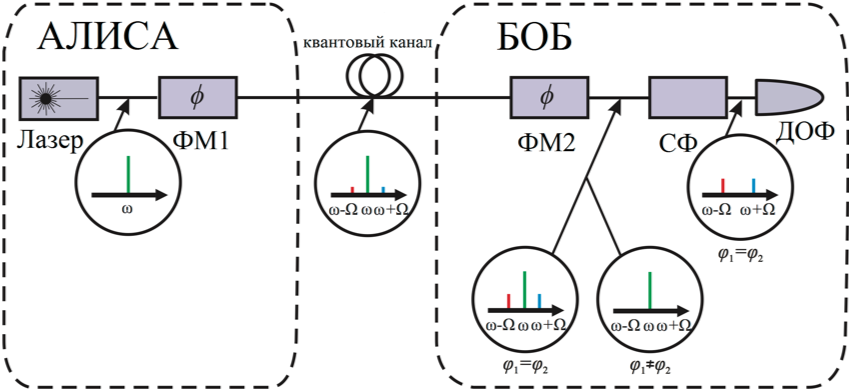
\includegraphics {Fig_3.png}
  \caption{Принципиальная схема ККБЧ}
  \label{fig:Fig_3}
\end{figure}


%%%%%%%%%%%%%%%%%%%%%%%%%%%%%%%%%%%%%%%%%%%%%%%%%%%%%%%%%%%%%%%%%%%%%%%%%%%%%%%%%%%%%%%%%%%%%%%%%%%%%%%%%%%%%%%%%%

\section{Измерительное оборудование в системах квантовой коммуникации} \label{sec:ch1/sec5}


Системы квантовой коммуникации (СКК) оперируют с низкоинтенсивным излучением в волоконно-оптических линиях связи (ВОЛС), где в среднем в каждом тактовом отсчете сосредоточена энергия не более одного фотона. Детекторы одиночных фотонов (ДОФ) способны улавливать подобные сигналы, что делает их неотъемлемой частью СКК. Условно ДОФ можно разделить на две группы: широкодоступные и узкоспециализированные. Очевидно, что детекторы из второй группы, например, криогенные термоэлектрические детекторы (QVD) [17] и детекторы, основанные на поглощении в холодном атомном паре [18], не могут быть использованы серийно в производстве систем СКК. Поэтому в данном разделе рассматриваются основные виды которые широко применимых ДОФ:

\begin{enumerate}
	\item использующие нанопроволоку в условиях сверхпроводимости (superconducting nanowire single-photon detector, SNSPD);
	\item на базе полевого транзистора, обогащенного квантовыми точками, с оптическим затвором (quantum-dot optically gated field-effect transistor, QDOGFET);
	\item на основе регистрации лавинных срабатываний при подаче большого обратного напряжения смещения на лавинный фотодиод (single-photon avalanche diode, SPAD);
	\item использующий джозефсоновский переход (superconducting-tunnel-junction detector, STJ);
	\item использующие сенсор, чувствительный к переходу материала из сверхпроводящего состояния в проводящее (transition-edge sensor, TES);
	\item счетчик фотонов видимого света (visible-light photon counter, VLPC) и твердотельный фотоумножитель (solid-state photomultiplier, SSPM).
\end{enumerate}

На основании сравнительной характеристики будет оценена целесообразность использования данных ДОФ для СКК.


\subsection{ДОФ, использующие сверхпроводящую нанопроволоку} \label{subsec:ch1/sec5/sub1}

Такой тип детекторов однофотонного излучения является одним из самых быстродействующих. Он способен регистрировать одиночные фотоны с частотой следования до нескольких гигагерц [21]. Основным элементом здесь служит площадка со сверхпроводящей тонкой проволокой (superconducting nanowire), запитанная током немного меньшим, чем критический, выше которого волокно выходит из сверхпроводящего режима. В таком случае поглощенный фотон оставляет небольшой участок нагретым и, соответственно, в проводящем состоянии. Поэтому ток начинает огибать этот участок с нормальной проводимостью. В результате ток превышает критическое значение, что приводит к переходу в проводящий режим всего участка. Появление участка с сопротивлением выражается в соответствующем скачке напряжения во внешней цепи, что и свидетельствует о детектировании фотона. Поскольку данный механизм детектирования требует очень узкой проволоки (порядка ~100 нм), его складывают меандром, для создания эффективной рабочей поверхности. Для повешения квнатовой эффективности детектирования (доля излучения, которая успешно переведена в электрический сигнал и зарегистрирована), сверху волокно покрывают отражающей поверхностью, в результате чего образуется резонатор, значительно повышающий эффективность детектора. В подобных устройствах используют в основном проволоку из нитрида ниобия, однако из-за высокого коэффициента отражения у данного материала - необходимо просветляющее покрытие, благодаря которому можно добиться высокого значения квантовой эффективности до 60-70 \%. Ввиду того, что детектор работает в сверхпроводящем режиме, ему необходимы низкие рабочие температуры менее 4 К. В таком режиме приёмное устройство характеризуется низким уровнем темновых срабатываний ($10^{-2}$-$10^2$ Гц).

\subsection{ДОФ, использующий полевой транзистор, обогащенный квантовыми точками, с оптическим затвором} \label{subsec:ch1/sec5/sub2}

Совмещение полевого транзистора с оптическим затвором из квантовых точек, расположенных между стоком и истоком, позволяют добиться регистрации одиночных фотонов инфракрасной области спектра [20]. Квантовые точки захватывают заряженные частицы, рожденные падающим светом, изменяя приложенное электрическое поле, что ведет к изменению протекающего по транзистору тока - по данному изменению и производится регистрирование сигнала. Впрочем, низкое быстродействие данного детектора не соответствует типовым системам СКК. Квантовая эффективность не превышает 15~\%, а максимальная тактовая частота следования квантовых сигналов составляет всего 50 кГц. Кроме того, для работы данного ДОФ необходимы низкие рабочие температуры (от 70 К и ниже). При этом вероятность темновых срабатываний характеризуется достаточно высоким значением.

\subsection{Лавинные фотодиоды для однофотонного излучения} \label{subsec:ch1/sec5/sub3}

Однофотонные детекторы этого типа используют процесс, схожий с тем, что происходит в фотоумножителе [19]. В отличие от фотоумножителя, в фотодиоде поглощение фотона рождает электрон-дырочную пару, которая порождает аналогичное увеличение числа заряженных частиц благодаря напряжению, приложенному вдоль кристаллической решетки полупроводника. Лавинные фотодиоды, используемые для оптического излучения в инфракрасном диапазоне, имеют низкие типичные показатели квантовой эффективности 10-25~\%. Они также характеризуются достаточно высокими значениями частоты темновых срабатываний (ложные срабатывания детектора в отсутствие входящего излучения, зачастую вызванного теплом окружающей среды), поэтому диод охлаждают до 210-250 К, например, термоэлектрическими охладителями. Даже в этом случае уровень темновых отсчётов для коммерческих ДОФ данного типа составляет порядка 1-10 кГц. Для лавинных детекторов характерна остаточная пульсация, когда электроны из лавины ненадолго <<застревают>>, например, в дефектах и, освобождаясь, порождают вторичные лавины. Необходимо некоторое время для выхода в штатный режим работы, поэтому у таких диодов обычно относительно высокое мертвое время (время, когда детектор сразу после срабатывания не может повторно зарегистрировать сигнал), что может ограничить тактовую частоту следования квантовых сигналов в СКК.), что важно при реализации дальнодействующих СКК.

\subsection{ДОФ, использующие джозефсоновский переход} \label{subsec:ch1/sec5/sub4}

Основным элементов для данного типа детекторов служит джозефсоновский переход - две части сверхпроводника разделенных сверхтонким (порядка 1 нм) диэлектриком, см., например, [22]. Квант света, падающий на сверхпроводящую область, вызывает распад большого числа куперовских пар электронов (квазичастицы), т.\:к. его энергия в тысячи раз больше энергии связи. Свободные электроны после распада пар способны туннелировать через диэлектрик во вторую часть сверхпроводника с крайне высокой вероятностью. Поскольку рабочая температура детектора на порядок ниже переходной температуры в сверхпроводящее состояние, куперовских пар распавшихся за счет иных процессов, нежели за счет поглощенных сигнальных фотонов, значительно меньше, что позволяет однозначно зарегистрировать однофотонное излучение. Таким образом, данный вид детекторов позволяет детектировать фотоны с эффективностью, не превышающей 45~\%, частотой следования фотонов порядка десятков кГц, однако при крайне низких рабочих температурах 0,37 К.

\subsection{Детекторы одиночных фотонов, использующий датчик, реагирующий на переход материала из сверхпроводящего состояния в проводящее} \label{subsec:ch1/sec5/sub5}

Данный сенсор работает по принципу болометра: при поглощении излучения повышается температура сенсора [23]. Для достижения чувствительности к одиночным фотонам необходима крайне малая теплоемкость поглощающего материала, и температурный датчик должен обладать чрезвычайно высоким откликом на малое изменение температуры. Это возможно при изготовлении датчика из тонкого сверхпроводящего материала, и его работы точно при температуре перехода из сверхпроводящего режима в обычный (порядка 100 мК) так, что небольшое изменение температуры отражается в значительном изменении сопротивления. Большей точности измерения колебаний сопротивления можно добиться, используя сверхчувствительный магнитометр, основанный на сверхпроводящем квантовом интерферометре (SQUID). Данный вид детекторов обладает самым большим показателем квантовой эффективности среди прочих - 95~\% для фотонов в ИК области. Несмотря на это, максимальная частота следования фотонов ограничена порогом в 100 кГц.

\subsection{ДОФ видимого света и твердотельный фотоумножитель} \label{subsec:ch1/sec5/sub6}

Величина квантовой эффективности данного детектора в области видимого света достигает 90~\% [24]. Принцип работы схож с лавинным диодом, но в данном случае не электрон, а дырка, выбитая падающим излучением, ускоряется к легированной части полупроводника, где уже рождает электронную лавину. Несмотря на высокое значение квантовой эффективности, остальные параметры достаточно низки: частота темновых срабатываний достаточно большая - не менее 20 кГц, максимальная скорость детектирования фотонов не превышает 100 кГц. Схожими по конструкции и принципу работы являются твердотельные фотоумножители [25]. Они обладают широкой спектральной восприимчивостью, что, в свою очередь, требует экранирования от дальнего ИК излучения, которое не представляет интереса.

\subsection{Cравнительная характеристика ДОФ для СКК} \label{subsec:ch1/sec5/sub7}

Ниже представлена таблица 1, в которой представлены ключевые параметры детекторов, описанных в предыдущих разделах.

\begin{table} [htbp]
	\centering
	\caption{Сравнительные характеристики распространённых ДОФ.}
	\label{tab:SPD_compare}
	\begin{tabular}{| c | c | c | c | c |}
	
	 \hline \makecell{Тип \\детектора} & \makecell{Рабочая T,\\~K} & \makecell{Квантовая \\эффективность,\\~\%} & \makecell{Максимальная \\частота \\регистрации \\квантовых \\сигналов} & \makecell{Темновые отсчеты, \% \\(от частоты \\регистрации \\квантовых \\сигналов)}   \\ \hline
	  SPAD         & 210-250    & < 25    & 300 МГц     & < 0,1   \\ \hline
	  STJ	   	   & < 1        & > 45    & 10 кГц  	& < 0,1      \\ \hline
	  QDOGFET      & < 80       & < 15    & 50 кГц      & < 1       \\ \hline
	  TES          & < 0,1      & > 90    & 1 МГц       & < 0,01       \\ \hline
	  \makecell{VLPC\\/SSPM} & < 10      & < 90    & 100 кГц       & < ~20      \\ \hline
	  SNSPD          & < 4      & < 60    & 3 ГГц       & < 0,0001       \\ \hline
	  
	\end{tabular}
\end{table}

На основе выполненного сравнения можно сделать следующие выводы. 


Лавинные фотодиоды для однофотонного излучения (SPAD) рекомендуется применять для систем квантовой коммуникации. Это объясняется тем, что они работают при нормальных температурах, которые возможно обеспечить без дополнительного охлаждающего криогенного оборудования, имеют оптоволоконный интерфейс и обладают максимальной частотой регистрации квантовых сигналов сопоставимой с  предполагаемой частотой смены квантовых состояний в типовых системах квантового распределения ключей. Относительно низкая квантовая эффективность и высокий уровень темновых срабатываний, однако, позволяет использовать данный вид детекторов на малых и средних дистанциях при небольших потерях в линиях ВОЛС (<15 дБ).


ДОФ, на основе джозефсоновского перехода (STJ) не рекомендуется использовать для приложений СКК ввиду низкой максимальной частоты регистрации одиночных фотонов и крайне низких рабочих температур, обеспечение которых является сложным технологическим процессом.


ДОФ, использующий полевой транзистор, обогащенный квантовыми точками, с оптическим затвором (QDOGFET) не рекомендуется использовать для приложений квантовых комуникации ввиду низкой максимальной скорости срабатывания.


ДОФ, использующий сенсор, реагирующий на переход материала из сверхпроводящего состояния в проводящее (TES) не рекомендуется использовать для приложений систем квантовой коммуникации ввиду низкой максимальной частоты регистрации квантовых сигналов и крайне низких рабочих температур, обеспечение которых является сложным технологическим процессом.


Счетчик фотонов видимого света (VLPC) и твердотельный фотоумножитель (SSPM) не рекомендуется использовать для приложений СКК по причине низкой скорости срабатывания. Также передача световых импульсов по ВОЛС накладывает ограничение на спектральный диапазон этих импульсов (ИК), ввиду чего применение счетчиков видимого света не оправдано.


ДОФ, использующий сверхпроводящую нанопроволоку (SNSPD) рекомендуется использовать для приложений СКК, т.\:к. они работают при температурах жидкого гелия (< 4K). Таке требования свою очередь компенсируется высокими ключевыми параметрами, которые обеспечат эффективную работу системы квантовой коммуникации. Данный тип детекторов следует использовать в каналах с относительно высокими потерями (от 15 дБ). 

%%%%%%%%%%%%%%%%%%%%%%%%%%%%%%%%%%%%%%%%%%%%%%%%%%%%%%%%%%%%%%%%%%%%%%%%%%%%%%%%%%%%%%%%%%%%%%%%%%%%%%%%%%%%%%%%%

\section{Атаки злоумышленника} \label{sec:ch1/sec6} 

В действительности существует значительное отличие между моделями, которые используются для теоретического подтверждения возможности формирования абсолютно стойких ключей квантовыми методами, и практическими реализациями таких систем. Во втором случае всегда существует малая вероятность того, что система или устройства будут иметь отклонение от усредненных параметров. Другим важным фактором является то, что компоненты таких систем зачастую не разрабатывались специально под данную задачу и поэтому потенциально могут иметь ряд других режимов, характеристик и свойств в других условиях и для применения в изначальных целях. Этими нюансами может воспользоваться злоумышленник, который хочет вопреки ограничениям остаться незамеченным и при этом получить максимальное количество ключевой информации. Известны ряд неидеальностей, которые, если их не учитывать, позволяют злоумышленнику добиваться значительных результатов. Такой подход и используемые для этого методы называются \textit{квантовым взломом} (quantum hacking). Это могут быть атаки злоумышленника с разделением пучка фотонов, формируемого в результате ослабления когерентного лазерного излучения, в котором статистика числа фотонов в импульсе подчиняется распределению Пуассона. Это значит, что существует ненулевая вероятность обнаружить в одном импульсе многофотонные состояния, отделить часть энергии и зафиксировать квантовое состояние, оставшись незамеченным. Другим потенциально уязвимым звеном систем квантовой коммуникации является детектор одиночных фотонов. Ниже обосновывается уязвимость систем при использовании таких устройств и возможные типы атак злоумышленника с использованием данной уязвимости. 

%	\subsection{Атака с разделением пучка фотонов}  \label{subsec:ch1/sec6/sub1}


%	\subsection{Атака типа перехват} \label{subsec:ch1/sec6/sub2}


%	\subsection{Атака типа перехват-пересылка} \label{subsec:ch1/sec6/sub3}


\subsection{Атака на детектор на основе ЛФД} \label{subsec:ch1/sec6/sub4}

Первым этапом проведения атаки с навязыванием ключа является определение возможности выведения детектора из режима счета фотонов (режима Гейгера). Известно, что вольт-амперная характеристика лавинного фотодиода имеет вид, представленный на рисунке \ref{fig:APDs_VA}.    

 \begin{figure}[ht]
  \centering
  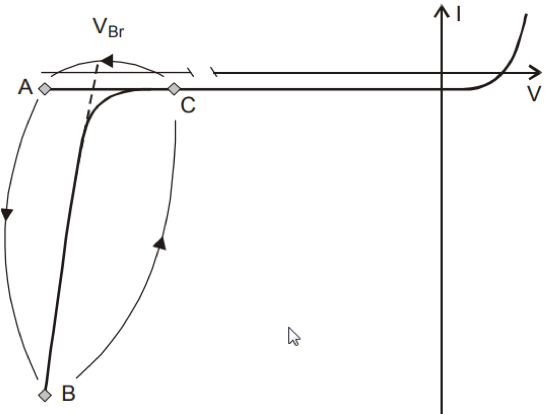
\includegraphics{APDs_VA.png}
  \caption{Вольт-амперная характеристика ЛФД}
  \label{fig:APDs_VA}
\end{figure}


Лавинный фотодиод работает при обратном напряжении смещения $-V_{bias}$ близком к напряжению пробоя $-V_{breakdown}$. Типичная величина находится в диапазоне от -40~В до -60~В. При величине обратного напряжения смещения ниже напряжения пробоя ЛФД находится в линейном режиме, где величина фототок $I_{APD}$ линейно зависит от падающей оптической мощности. При увеличении величины обратного смещения выше напряжения пробоя ЛФД переходит в режим счета фотонов, или режим Гейгера. В этом режиме даже энергии единиц фотонов достаточно для формирования лавины зарядов и резкого скачка фототока. При превышении некоторого порогового значения $I_{det}$, регулируемого уровнем срабатывания компаратора, формируется электрический импульс, который и интерпретируется, как регистрация одиночного фотона. 

 \begin{figure}[ht]
  \centering
  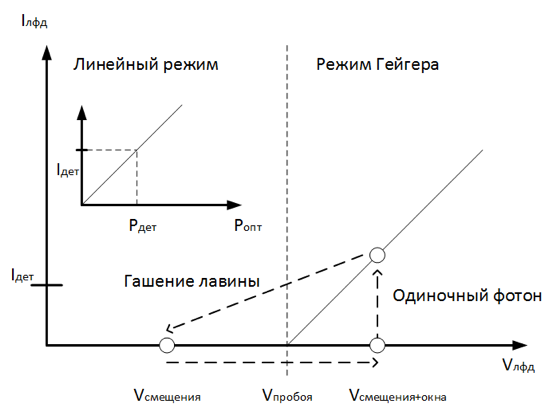
\includegraphics{Vbreakdown}
  \caption{Граница между режимами работы ЛФД при подаче обратного напряжения смещения}
  \label{fig:Vbreakdown}
\end{figure}

Гашение лавины в самом простом случае происходит благодаря последовательно подключенному в цепь резистору, как показано на рисунке \ref{fig:Quenching}. Существуют также схемы активного гашения лавины.  

 \begin{figure}[ht]
  \centering
  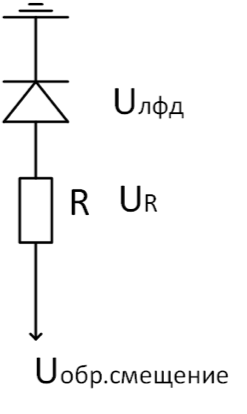
\includegraphics{Quenching}
  \caption{Принципиальная электрическая схема подключения ЛФД для регистрации одиночных фотонов}
  \label{fig:Quenching}
\end{figure}


Для снижения уровня шумов срабатываний ДОФ на базе ЛФД функционируют в режиме стробирования, когда в момент ожидаемого прибытия фотона на диод подается дополнительное напряжение в форме импульса, т.\:н. окно срабатывания $-V_{gate}$, величиной около 3~В. Благодаря этому импульсу диод переходит из линейного режима при величине напряжении $-V_{bias}$, в котором он прибывает относительно длительное время порядка единиц микросекунд, в режим счета фотонов, где $-V_{bias+gate} < - V_{breakdown}$.  

\subsection{Атака с навязыванием ключа ( Faked-state attack)} \label{subsec:ch1/sec6/sub5}


В работе показана полноценная реализация атаки с использованием уязвимости детектора на основа ЛФД. Злоумышленник имеет модифицированный приёмный узел, аналогичный блоку получателя м связанный с модифицированным узлом отправителя. Первый принимает квантовые состояния от легитимного отправителя и те случаи, где происходит совпадения посылает в модифицированный узел отправителя. Там используется интенсивное оптическое излучение для контроля детектора фотонов и формирования срабатываний в требуемых злоумышленнику отсчетах. Таким образом, он является незамеченным обладателем ключевой информации. 

 \begin{figure}[ht]
  \centering
  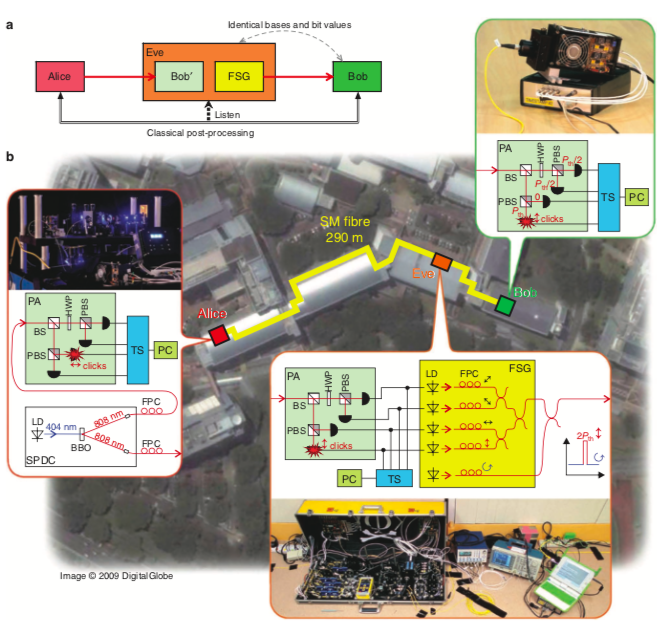
\includegraphics[scale=0.5]{FSA.png}
  \caption{Принципиальная схема проведения атаки с поддельными состояниями}
  \label{fig:FSA}
\end{figure}

\pagebreak
%%%%%%%%%%%%%%%%%%%%%%%%%%%%%%%%%%%%%%%%%%%%%%%%%%%%%%%%%%%%%%%%%%%%%%%%%%%%%%%%%
%	\subsection{Атака на SNSPD} \label{subsec:ch1/sec6/sub6}


%%%%%%%%%%%%%%%%%%%%%%%%%%%%%%%%%%%%%%%%%%%%%%%%%%%%%%%%%%%%%%%%%%%%%%%%%%%%%%%%%%%%%%%%%%%%%%%%%%%%%%%%%%%%%%%%%%

\section{Известные контрмеры против атак на измерительное оборудование} \label{sec:ch1/sec7}

Существует ряд решений для предотвращения атаки с навязыванием ключа. Ниже перечислены основные. Однако, следует отметить, что строгое доказательство секретности, а также многочисленные экспериментальные работы, подтверждающие практическую ценность есть только у предпоследнего подхода. Остальные контрмеры требуют исследования в стенах лабораторий, практикующих квантовый взлом. 

\subsection{Статистика счета фотонов} \label{subsec:ch1/sec7/sub1}

В работе предложена контрмера, основанная на наборе статистики фотонов, которые поступают на светоделитель с двумя детекторами. В случае применения атаки с <<ослеплением>> изменяется количество одновременных совпадений на этих двух детекторах относительно их нормального режима работы. 

 \begin{figure}[ht]
  \centering
  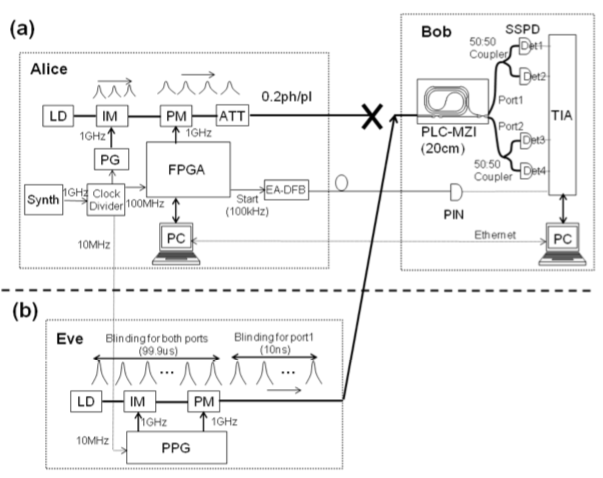
\includegraphics[scale=0.5]{PhotonStatistics.png}
  \caption{Принципиальная схема контрмер на основе статистики фотонов}
  \label{fig:PhotonStatistics}
\end{figure}

\subsection{Измерение фототока} \label{subsec:ch1/sec7/sub2}

Очевидным решением является активный мониторинг фототока, протекающего в ЛФД при попадании на него оптического излучения, и наблюдении лавинного пробоя, как показано на рисунке \ref{fig:Photocurrent}. 

 \begin{figure}[ht]
  \centering
  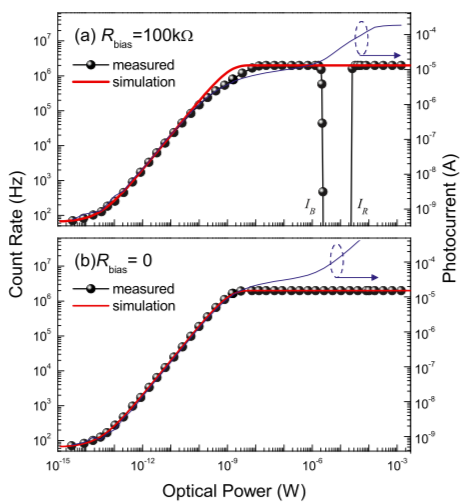
\includegraphics[scale=0.5]{Photocurrent.png}
  \caption{Зависимость количество отсчетов и фототока от интенсивности падающего излучения}
  \label{fig:Photocurrent}
\end{figure}
\pagebreak

\subsection{MDI-протокол} \label{subsec:ch1/sec7/sub3}

В работе предложен метод, в основе которого лежит предположение о том, что измерительный узел доступен злоумышленнику, который при этом знает какие из детекторов произвели срабатывание и в какой временной отсчет, однако при этом не имеют информации о том, какое квантовое состояние в блоках Алисы и Боба применялось. Это достигается за счет интерференции слабых когерентных импульсов на светоделителе внутри недоверенного узла регистрации. В процессе постселекции легитимные пользователи выявляют результат однофотонной интерференции, который привел к срабатыванию, и соотвествующие ему состояние, которые были использованы. Такой подход получил название MDI (measuerement-device-independent) и нашел широкое применение для исследований, благодаря устойчивости к атакам на измерительное оборудование. Однако, на практике ввиду чрезвычайному усложнению оптической схемы и условий, при которых наблюдается интерференция, почти не применяется в условиях близких к реальным. 


 \begin{figure}[ht]
  \centering
  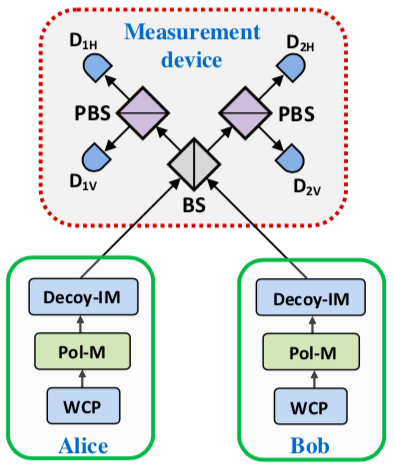
\includegraphics[scale=0.5]{MDI_scheme.png}
  \caption{Принципиальная схема системы с независимым измерительным устройством MDI}
  \label{fig:MDI_scheme}
\end{figure}


\subsection{Twin-Field протокол} \label{subsec:ch1/sec7/sub4}


Развитием темы MDI с применением фазовых состояний является протокол Twin-Field (близнецовые поля), где так же применяется анонсирование измерительным узлом, доступным злоумышленнику, результата интерференции когерентных состояний на светоделителе, которые приводят к срабатыванию детекторов одиночных фотонов. Отличительной особенностью является то, что в отличие от MDI, где для минимизации корреляции по фазе последовательности импульсов от каждого из источников, используется их рандомизация, то есть изменение фазы случайным образом, в протоколе Twin-Field используется результат интерференции когерентных состояний с определением секторов на фазовой плоскости и отбрасыванием фазовых состояний, соответствующих разным секторам в процессе постобработки.

 
 \begin{figure}[ht]
  \centering
  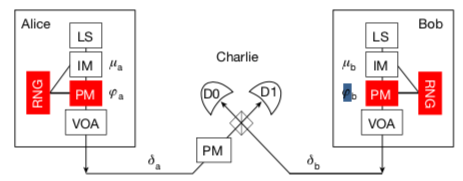
\includegraphics[scale=0.5]{TF_scheme.png}
  \caption{Принципиальная схема системы с независимым измерительным устройством}
  \label{fig:TF_scheme}
\end{figure}
%%%%%%%%%%%%%%%%%%%%%%%%%%%%%%%%%%%%%%%%%%%%%%%%%%%%%%%%%%%%%%%%%%%%%%%%%%%%%%%%%%%%%%%%%%%%%%%%%%%%%%%%%%%%%%%%%%

\section{Выбор направления исследований. Цели и задачи работы} \label{sec:ch1/sec8}

Системы ККБЧ зарекомендовали себя, как перспективное направление коммерчески доступных устройств квантового распределения ключа с практически значимыми характеристиками мирового уровня, подтвержденными в ряде научных публикаций в международных изданиях, формализованным доказательством безусловной секретности используемого протокола, применением на нескольких полигонах, развернутых на территории Российской Федерации, совместно с ведущими компаниями в области телекоммуникационной связи, банковского сектора и региональными инжиниринговыми центрами. 


С научной и инженерной точки зрения данный класс систем имеет большой задел:

\begin{enumerate}
	\item Экспериментальная демонстрация передачи квантовых состояний на основе технологии квантовой коммуникации на боковых частотах модулированного излучения в телекоммуникационной линии связи с потерями, соответствующими дальности свыше 250 км [?]. 
	\item Была проведена разработка функциональной схемы и экспериментальная реализация оптико-электронного устройства квантовой передачи информации на боковых частотах, включающую подсистему непрерывной синхронизации модулей отправителя и получателя, подсистему компенсации неконтролируемого изменения поляризации в оптическом волокне [?].
	\item Экспериментально продемонстрировано спектральное уплотнение каналов на боковых частотах [?]. 
	\item Экспериментальная демонстрация применимости данной технологии для квантового распределения ключа в открытом пространстве, а не только в волоконно-оптических линиях связи [?]. 
\end{enumerate}


Однако, устойчивость квантовых систем передачи информации на боковых частотах к воздействию нелегитимного пользователя на измерительной оборудование ранее не была исследована. 


{\aim} данной работы является исследование возможностей злоумышленника по получению секретного ключа с использованием атак на измерительное оборудование систем квантовой коммуникации на боковых частотах и разработка методов противодействия атакам.


Для~достижения поставленной цели ставились следующие {\tasks}:
\begin{enumerate}
  \item Исследование устойчивости детектора одиночных фотонов, применяемого в системах квантовой коммуникации на боковых частотах, к атакам с выведением из режима Гейгера (<<ослеплением>>). 

  \item Оценка возможностей злоумышленника при атаке с выведением из режима Гейгера для систем квантовой коммуникации на боковых частотах. 

  \item Разработка оптической схемы системы квантовой коммуникации, устойчивой к атакам на измерительное оборудование. 

  \item Разработка протокола квантовой рассылки ключа, устойчивого к атаке на измерительное оборудование. 

\end{enumerate}
